
%%%%%%%%%%%%%%%%%%%%%%%%%%%%%%%%  ejemplo.tex %%%%%%%%%%%%%%%%%%%%%%%%%%%%%%%

%%%%% Fichero de ejemplo LaTeX que ilustra el uso de la Hoja de Estilo %%%%%%
%%%%% Jornadas.cls para las XXII Jornadas de Paralelismo.              %%%%%%

\documentclass[twocolumn,twoside]{Jornadas}
\usepackage{fontspec}
\usepackage{xunicode}
\usepackage{xltxtra}
\usepackage{graphicx}
\graphicspath{{imgs/}}

\usepackage{listings}
\usepackage{color}
\lstloadlanguages{Python}
\lstset{
  language=Python,                      % C,Fortran,XML
  basicstyle=\scriptsize,               % Listados en small
  keywordstyle=\color{red},             % Palabras clave en rojo
  identifierstyle=\ttfamily,
  escapeinside={(*@}{@*)},
  commentstyle=\color{blue},            % comentarios en azul
  stringstyle=\color{green},            % cadenas en verde
  showstringspaces=false,
  frame=tb,
  captionpos=t,
  belowcaptionskip=12pt,
  stepnumber=2,                                         % Opciones de lineas y etiquetas
  numberstyle=\scriptsize,
  numbersep=5pt,
  tabsize=1
}


%%%%%%%%%%%%%%%%%%%%%%%%%%%%%%%%%%%%%%%%%%%%

\begin{document}


\title{Experiencias con Python y CUDA en Computación de Altas Prestaciones}

\author{Sergio Armas,%
     Lionel Mena,%
     Alejandro Samarín,% 
     Vicente Blanco%
     \thanks{Dpto. Estadística, I.O. y Computación, Univ. La Laguna, e-mail: {\tt vblanco@ull.es}},%
     Alberto Morales y % 
     Francisco Almeida
}

\maketitle
% Oculta las cabeceras y los números de página.
% Ambos elemetos se añadirán durante la edición de las actas completas.
\markboth{}{}
\pagestyle{empty} 
\thispagestyle{empty} % Oculta el número de la primera página

\begin{abstract}

\end{abstract}

\begin{keywords}
Python, CUDA, 
\end{keywords}

\section{Introducción}

\ldots utilizando PyCUDA~\cite{DBLP:journals/corr/abs-0911-3456}

y una gráfica \ref{fig:Fermi}

\begin{figure}
	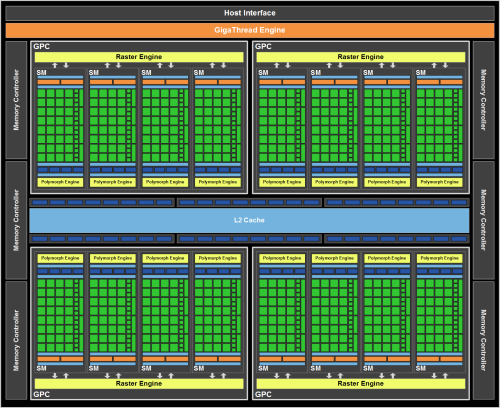
\includegraphics[width=.45\textwidth]{block_diagram_Fermi}
	\caption{\label{fig:Fermi} Diagrama de bloques de una GPU Tesla M2070 (Fermi)}
\end{figure}

y un código \ref{code:filter}

\lstinputlisting[%
   float=t,
   caption={Codigo de filtros en Python},
   label={code:filter} 
   ]%
   {code/filter.py}

\bibliographystyle{Jornadas}
\bibliography{pycuda}

\end{document}

